\documentclass[12pt, letterpaper]{article}
\usepackage{enumitem}
\usepackage[utf8]{inputenc}
\usepackage{amsmath}
\usepackage{array}     
\usepackage{booktabs}   
\usepackage[table]{xcolor}


% ==========================================
% 1. PAPER SIZE & MARGINS
% ==========================================
\usepackage[letterpaper, left=1.5in, top=1in, right=1in, bottom=1in]{geometry}
\usepackage{microtype} 
\usepackage{caption}
\usepackage{float}
\usepackage{longtable}   % allows tables to break across pages
\usepackage{booktabs}    % provides professional spacing and rules
\usepackage{array} 
\usepackage{pdflscape}   % landscape with PDF rotation
\usepackage{graphicx}    % for images
\usepackage{listings}    % for code blocks (optional)
\usepackage{caption}     % for better caption control


% ==========================================
% 2. SPACING & ALIGNMENT
% ==========================================
\usepackage{setspace}
\singlespacing 

% ==========================================
% 3. LANDSCAPE PAGES (For Diagrams)
% ==========================================
\usepackage{pdflscape}

% ==========================================
% 4. FONTS (Using Uploaded Files)
% ==========================================
\usepackage{fontspec}

% Tell LaTeX to look in the current folder (Path = ./) 
% and specify the EXACT filename of the Century font you uploaded.
\setmainfont{Century.ttf}[
    Path = ./,
    % If you uploaded separate files for bold and italics, you can add them like this:
    % BoldFont = CenturyBold.ttf,
    % ItalicFont = CenturyItalic.ttf
]

% Specify the EXACT filename of the Century Schoolbook font you uploaded.
\newfontfamily\titlefont{Century.ttf}[
    Path = ./
]

\usepackage{titlesec}
% Format Sections to match the outline (Section I - Introduction)
\titleformat{\section}{\titlefont\fontsize{12}{14.4}\selectfont\bfseries}{ \Roman{section} - }{0em}{}
\titleformat{\subsection}{\titlefont\fontsize{12}{14.4}\selectfont\bfseries}{\thesubsection}{1em}{}
\titleformat{\subsubsection}{\titlefont\fontsize{12}{14.4}\selectfont\bfseries}{\thesubsubsection}{1em}{}

% ==========================================
% 5. CUSTOM TITLE FORMAT (Inverted Triangle)
% ==========================================
\newcommand{\invertedtitle}[1]{
    \begin{center}
        \titlefont\fontsize{17}{20.4}\selectfont\bfseries
        #1
    \end{center}
}

% ==========================================
% 6. Check and x marks.
% ==========================================
\usepackage{amssymb} % Required for the \checkmark symbol
\usepackage[numbers]{natbib}
\usepackage{booktabs}
\usepackage{tabularx}
\usepackage{graphicx}
\renewcommand{\figurename}{Fig.}
\begin{document}

% ------------------------------------------
% MANUSCRIPT HEADER
% ------------------------------------------

% 1. The Title 
% (Uses the \invertedtitle command. Instruct students to use \\ to break 
% lines so that each line is shorter than the one above it.)
\invertedtitle{
    Weld Track: An Inventory Management System for Goboles’s Welding Shop with Cost Tracking 
}

\vspace{1.5em}

\begin{center}
    % 2. Authors (Century, 12pt)
    {\fontsize{12}{14.4}\selectfont
    Dave Angelo P. Gelilio\textsuperscript{}, Joram H. Hona\textsuperscript{}, John carl S. Gobole\textsuperscript{}, Louie jay Arthur S. Rogacion\textsuperscript{} \par}
    
    \vspace{1em}
    
    % 3. Affiliation (Century, 12pt)
    {\fontsize{12}{14.4}\selectfont
    College of Information and Communications Technology \\
    Sorsogon State University - Bulan Campus \\
    Bulan, Sorsogon \par}
    
    \vspace{1.5em}
    
    % 4. Emails (Century, 12pt)
    {\fontsize{12}{14.4}\selectfont
    E-mails: geliliodaveangelo996@gmail.com ;gobolejohncarl2929@gmail.com; joramhona520@gmail.com;rogacionlouie@gmail.com\par}
\end{center}

\vspace{2.5em} % Adds space between the header and the executive summary

% ------------------------------------------
% EXECUTIVE SUMMARY
% ------------------------------------------
\begin{center}
    {\titlefont\fontsize{12}{14.4}\selectfont\bfseries Executive Summary}
\end{center}
\newpage % Pushes Section I to the next page

% ------------------------------------------
% SECTION I
% ------------------------------------------
\section{Introduction}
 \hspace*{2em}This section will discuss the proposed project, detailing the context of the welding shop, the problems it faces with its current manual inventory and costing methods, the purpose of the proposed system, its objectives, and the scope and boundaries of the project
\subsection{Project Context}
 \hspace*{2em}Inventory management is one of the most critical components of businesses that monitors and tracks physical supply, from purchasing to manufacturing. Incompetent inventory tracking and management can lead to notable financial losses due to waste materials, loss of materials, theft, project delays due to stockouts, and cost estimation error for projects. For small and medium-sized businesses, especially for those specialized in trades and product fabrication like welding shops, the absence of affordable and user-friendly digital tools often constraints them to rely on traditional manual methods, using pen and paper for logs or basic recordings, which can lead to human error, data redundancy, and loss of data. A transformative digital platform for welding and fabrication shops, moving them away from outdated manual processes and isolated data toward becoming integrated, data-driven. Traditional welding operations often struggle with challenges such as material waste, inefficient scheduling, and an inability to meet strict industry traceability requirements (like ISO or NADCAP) using legacy tools or spreadsheets. By replacing these fragmented systems with a unified cloud-based ecosystem, Dynamics 365 provides real-time production insights through IoT integration, allowing shops to track weld arc time, manage complex multi-level Bills of Materials (BOM), and automate quality control [1].
\hspace*{2em} The welding industry, one of the most important in the product fabrication and construction sector, relies heavily on the availability of electrodes, gas, and equipment. In this country, Welding shops like Gobole's welding shops are commonplace. Offering services like fabrication and repairs for public communities. These small shops operate in a competitive environment where growth and profits depend on systematic use of materials and cost estimation of projects. The Department of Trade and Industry (DTI) supports the digital transformation of MSMEs to increase their operational efficiency and competitiveness in the modern economy. The main point of the sources is that the digital transformation of the welding and fabrication industry both in educational training and industrial operations is essential to overcome the high costs, inefficiencies, and quality limitations of traditional manual methods. By adopting to advanced technologies, integrated cloud platforms like Microsoft Dynamics 365 for production, the industry can move toward a "smart factory" model that is data-driven, flexible, and highly precise [2].

\newpage
\hspace*{2em} This software project is a web-based inventory management system for a small business enterprise established in Pagadian City, Zamboanga del Sur, Philippines. It primarily supports the business owner of the said business enterprise to perform regular inventory management online through a web platform. This mechanism did not only improve the overall business process but also enabled the business owner to manage inventories with efficiency and convenience. The enterprise comprises four branches and a mobile store that strolls around the city to cater to customer needs. In addition, the current mechanism of conducting inventory management is purely manual through the use of paper files, which overwhelmed the business owner with several challenges, including data inaccuracy due to the reliance on using papers where data are recorded and process inefficiency due to the manual recording and distribution of inventory and sales reports. This software project addressed these challenges by eliminating these manual approaches through an automated computing solution using a web platform where data are electronically recorded and processed, and reports are electronically produced [3].
\hspace*{2em} Gobole's Welding Shop, located in Sta. Remedies, Bulan, Sorsogon, is a local Welding shop business established in January 19, 2022. The Welding shop offers a variety of fabrication services, including building a tricycle, table and chair, motor and tricycle repair related to any metal/steel structure. Gobole's welding shop operations involves managing inventory of various steel profiles like angle bars, square tubes, flat bars, welding rods, grinding discs, cutting disc, and maintaining functional welding machines and power tools. The shop caters to walk-in customers and project-based contracts.
\hspace*{2em} The main problem at Gobole’s Welding Shop is the dependence on a manual system with no available system for managing inventory, project costs estimation, customer job orders, or appointments. Currently, supplies are tracked using a physical logbook, which often leads to manual errors and inconsistent updates. Determining the exact quantity of a specific supply remaining, for example, requires a physical count and a search through the logbook or rummaging through the entire inventory.
\hspace*{2em} When a new project is accepted by the owner, material costs and project cost estimation are based on experience, past projects, and memory, rather than accurate current inventory levels and current material prices in the market. This leads to inconsistent and unprofessional quotation generation. Moreover, there is no financial visibility into revenue, invoicing, or project profitability, and no ability to compare estimated project costs against actual expenses. Additionally, metal scrap sold to junk shops remains unaccounted for.
\hspace*{2em} Walk-in customers sometimes go to the shop without notifying the owner. They come to the shop and the owner is not around, which is a hassle for the customer and a waste of time and energy. The lack of a centralized system for managing customer job orders and appointments further worsens this issue.
\hspace*{2em}This project, Weldtrack, seeks to solve these problems by presenting a simple, user-friendly, convenient web-based system. By digitalizing inventory tracking and management, the Weldtrack will provide an overview of the shop's inventory status, appointment management, financial performance. The owner can manage appointments and date of the pick-up of the projects. The project helps the owner to give a confident and reliable decision, not just by predict.


\subsection{Purpose and Description}
\hspace*{2em}The main purpose of this capstone project is to design and develop "Weldtrack," which is a simple and user-friendly web-based inventory management system that tracks costs, especially for Gobole's Welding Shop. This capstone project seeks to replace the current manual logbook system used by the welding shop with a centralized application that will improve accuracy, increase efficiency, and provide valuable information for business management.
\hspace*{2em}The intention behind developing Weldtrack is to provide a tool for the business owner and employees that will improve how they currently manage their inventory. At its core, this application is meant to handle all the inflows and outflows of inventory, ensuring that all materials and tools used for various projects are carefully recorded and monitored. The development of this application is meant to provide key features that will satisfy the needs of the welding shop, such as providing a search record for all materials and tools, displaying current stock levels, and sending notifications when stock is running low. The core component of this application is its project-costing module, which will be used to log new welding jobs and enter materials used for each new project. This will automatically subtract materials from the inventory count, which will then determine.
\hspace*{2em}No centralized system for managing customer job orders and appointments - This leads to scheduling conflicts, missed customers, and disorganized project workflows
\hspace*{2em}Inconsistent and unprofessional quotation generation – Quotes are often based on guesswork rather than accurate material costs, resulting in lost revenue or customer dissatisfaction.
\hspace*{2em}No financial visibility into revenue, invoicing, or project profitability – The owner cannot identify which jobs are most profitable or track overall business performance.
\hspace*{2em}No ability to compare estimated project costs against actual expenses – This prevents the owner from learning from past projects and improving future cost estimates.
\hspace*{2em}Unaccounted metal scrap sold to junk shops – After project fabrication, leftover metal scraps are sometimes sold to junk shops, but these transactions are not recorded in the shop’s inventory or financial records. As a result, the shop loses potential revenue, inventory counts remain inaccurate, and there is no visibility into how much scrap value is being generated or lost.
\hspace*{2em}By implementing Weldtrack, the owner can make accurate decisions about re-stocking supplies, accurate estimation of cost of future projects based on usage of materials in the previous projects, and easily identify which projects generate the highest profit margins. This shift to visionary, data-centric decision-making means the owner no longer relies on gut feelings when pricing jobs like tricycle sidecar or motor repairs. Weldtrack estimates the normal material cost and labor time for those specific repairs, then automatically inputs current supplier prices to generate a highly accurate, profitable quote. This data-driven approach ensures every offer is consistent and profitable, while allowing the owner to predict inventory needs based on upcoming work, transforming the shop's operations from simple guesswork into a strategically managed, financially stable enterprise.
\hspace*{2em} The implementation of Weldtrack is to design and create a positive domino effect through Gobole's Welding Shop, directly benefiting the people who relate with the business every day. For the owner, the system provides complete, real-time visibility into operations, enabling strategic control over cash flow, data-backed pricing strategies, and the ability to identify the most profitable projects. Employees will enjoy a smooth workflow, replacing slow manual logbook entries with a quick and efficient digital process for logging materials.

\subsection{Objectives}
\hspace*{2em}This study aims to design, develop, and evaluate WeldTrack, a web-based inventory, booking, staff-work, and project-cost management information system for Gobole's Welding Shop. Specifically, it aims to:

\begin{enumerate}
    \item To develop a role-based booking and appointment-management module for customer requests, administrative approval and scheduling, and assigned staff work.
    \item To develop an inventory-management module with stock monitoring, material issuance, movement history, low-stock alerts, and insufficient-stock prevention.
    \item To develop automated project-cost calculation and completed-project revenue monitoring.
    \begin{enumerate}[label=\theenumi.\arabic*]
        \item Estimated labor-cost calculation from estimated hours and the configured service rate
        \item Actual labor- and material-cost calculation from recorded project work
        \item Backend-calculated final project price and completed-project revenue reporting
    \end{enumerate}
    \item To evaluate the system using ISO 25010 with the following indicators:
    \begin{enumerate}[label=\theenumi.\arabic*]
        \item Functional Suitability
        \item Performance Efficiency
        \item Interaction Capability
    \end{enumerate}
\end{enumerate}

\subsection{Scope and Limitations}
\hspace*{2em}WeldTrack is a responsive web-based management system for Gobole's Welding Shop with Administrator, Staff, and Customer roles. Customers manage addresses, browse services, submit and track bookings, view estimated and final project prices, cancel eligible pending requests, and provide feedback. Administrators manage services, booking approval and scheduling, staff assignments, inventory, attendance corrections, payroll, reports, and feedback moderation. Staff access assigned tasks, record attendance, labor hours and material usage, upload project images, and view personal payslips and contributions.
\hspace*{2em}During booking approval, an administrator records estimated labor hours and the system calculates estimated labor cost from the configured service hourly rate. Assigned staff later record actual labor hours and materials used. The backend calculates actual labor cost, material cost, and the final project price from persisted records. Completed project totals are summarized as operational revenue.
\hspace*{2em}WeldTrack does not replace accounting software and does not generate formal quotations, invoices, receipts, tax records, payment ledgers, or online-payment transactions. It also excludes weighted-average purchase costing, advanced scheduling optimization, CAD/CAM integration, complex supply-chain management, native mobile applications, and commercial round-the-clock support.

% ------------------------------------------
% SECTION II
% ------------------------------------------
\section{Review of Related Systems}
\hspace*{2em}This Section will examine the existing system that are related on WeldTrack: An Inventory Management System for Gobole’s Welding Shop with Cost Tracking. the purpose of this review is to establish a comprehensive understanding of how current inventory management and cost tracking solutions operate across different industries and more importantly, to identify the gaps and limitations that WeldTrack is specifically designed to address.

\subsection{Introduction to Related Systems}
   \hspace*{2em}This chapter presents a comprehensive review of related systems relevant to the development of WeldTrack: An Inventory Management System for Gobole’s Welding Shop with Cost Tracking. It will examine several existing systems, technologies, and web-based applications that are connected with inventory management, cost tracking, and business operation processes. The purpose of this chapter is to analyze how these systems function, identify their features, and evaluate their strengths and limitations in relation to the proposed system
\subsection{Overview of Each Related System}
   \hspace*{2em} The ALAR welding workshop specializes in metal fusion using various techniques, with a critical focus on material inventory management. Currently, manual recording of inventory leads to inaccuracies, delays, and difficulties in tracking. To address these issues, a web-based material inventory information system has been developed to streamline inventory management, replacing error-prone manual methods and enhancing operational efficiency. Employing a waterfall approach, the research involved a sequential design process Including needs analysis, system design, implementation, testing, and maintenance. Findings reveal that the system allows personnel to efficiently record, monitor, and report inventory in real-time, improving data accuracy and time efficiency. This system facilitates better decision-making for material procurement by providing current, precise data, representing an effective solution for ALAR Welding Workshop’s material management needs [4]. 
\hspace*{2em}Inventory managers globally face complex challenges in maintaining seamless manufacturing, delivering quality services, optimizing inventory levels, and enforcing effective inventory policies. As organizations grow, they encounter issues related to diverse inventory items that complicate tracking, necessitating a formal record-keeping system. Increased inventory demands more space, prompting businesses to enhance operations amidst local and global competition. Companies must adopt strategic inventory management to thrive, making intelligent systems crucial. This study introduces a web-based intelligent inventory management system that integrates multiple stores, ensuring effective coordination. It calculates reorder points for various stores and communicates them to a central location using Java Remote Method Invocation (RMI) with secure socket layer (SSL). Technologies such as MySQL, HTML, JavaScript, PHP, and Xampp facilitate this system. The research aims to improve inventory management performance by transitioning from a single-store model to a distributed system that accurately reflects real-time supplies across different locations [5].
\hspace*{2em}Internet technology encourages businesses to adopt digital systems that improve productivity and support data-driven decisions. However, PT. Jodo Global still uses manual inventory tracking, leading to problems like data inaccuracies and delays in reporting. This highlights the need for research, as a lack of a cohesive inventory system has harmed operational precision and management decisions. The research aims to create a web-based inventory management system for real-time stock tracking, organized transaction records, and automatic report generation. The development involved requirement analysis, system design, implementation, and functionality testing. Key capabilities tested included stock updates, transaction documentation, user verification, and report generation based on performance metrics such as accuracy and responsiveness. The results showed significant improvements, including a 60\% reduction in processing time, an 83\% decrease in recording errors, and fully automated report generation, enhancing efficiency and accuracy at PT. Jodo Global [6].
\hspace*{2em}Inventory is a crucial part of a systematic supply chain, yet small firms often neglect inventory management (IM) by accumulating excessive inventory over time. This study examines the IM practices of small and medium enterprises (SMEs) in Bangladesh using a qualitative case study design, with data collected from ten SME owners through semi-structured interviews analyzed via NVivo software. The findings reveal that most SME owners source raw materials from local markets, supplemented by international suppliers, while those dealing with recycled products procure materials from across the country. Digital technologies and online media are frequently used to manage raw materials, though financial constraints, wastage, and damage limit the volume of purchases, resulting in losses of 10–15\%. This research offers valuable insights for the government, the SME Foundation, and trade associations, recommending that import taxes on raw materials and export duties on finished products be reduced to better support SME inventory management [7]. 
\hspace*{2em}In any manufacturing industry, monitoring and managing the consumption of raw materials and goods is essential for maintaining operational sustainability and profitability. Amid intensifying global competition, manufacturers continuously seek inventory management systems that can reduce costs and shorten the lead time for supplying materials, thereby enabling faster and more efficient production. Consequently, ongoing refinement of existing inventory management approaches is crucial to remaining competitive. Although modern systems have significantly benefited from barcode technology, our research identifies an opportunity to enhance barcode-based designs by integrating them with cloud computing, Arduino-based wireless station nodes, the Internet of Things (IoT), and a secure web portal for data access. This paper presents a novel model that applies such integration to manage inventory of essential formwork shuttering products in the construction sector. While our study is grounded in the context of Indian construction companies, the findings and the proposed approach are potentially applicable to other regions as well [8].
\hspace*{2em}Inventory control is essential for business operations, including educational institutions. This research used a quantitative descriptive approach to study the University of Baguio Requisition, Procurement, and Inventory System (UBRPIS), which automates inventory management. The study aimed to evaluate employees’ understanding of inventory management, identify system weaknesses, and recommend improvements. Most respondents were familiar with UBRPIS procedures like requesting non-consumable goods and using barcodes. However, nearly half reported issues, with significant challenges related to barcode placement and a shortage of non-consumable items. Although users know the system, they face operational difficulties. The study suggests that the University should invest in better inventory technology and provide ongoing training for staff on UBRPIS [9].
\hspace*{2em}In order to help custodians manage their inventories effectively, inventory systems are essential to business and academic operations. To make inventory organizing and sorting more efficient, the BSIT students created a web-based inventory system. This system has characteristics. The institution used manual inventory procedures in the past, which involved handwritten documents that could be lost or damaged. Compared to the conventional methods, the novel technology greatly improves security and accuracy [10].
\hspace*{2em}Managing inventory for items with a limited shelf life is challenging because they spoil over time. This research is important for the operators of Convenience Store X in Marikina City and for future studies on inventory management systems. The goal is to create a user-focused inventory management system using a design thinking process that includes five stages: Empathize, Define, Ideate, Prototype, and Test. Researchers gathered information on the challenges users face with managing perishable items and created criteria for a new system. They used Multi-Criteria Decision Analysis (MCDA) and worked with developers to design three user interfaces for the inventory system, called System X, System Y, and System Z. User testing showed that System X was the preferred option [11].
\hspace*{2em}This software project is a web-based inventory management system developed for a small business based in Pagadian City, Zamboanga del Sur, Philippines. It is designed to help the business owner conduct inventory management online, streamlining operations and providing greater efficiency and convenience. The business operates four physical branches and one mobile store that travels around the city to serve customers. Prior to this system, inventory management was done manually using paper records, which led to several difficulties for the owner, such as inaccurate data due to reliance on handwritten logs and inefficiencies from manually recording and distributing inventory and sales reports. The project addressed these issues by introducing an automated, web-based solution that enables electronic data entry, processing, and report generation eliminating the previous manual processes [12]. 
\hspace*{2em}This study assessed the perceived financial performance of selected pharmacies in Baliwag City by evaluating the effectiveness, challenges, and benefits of their inventory management systems. It also examined whether significant relationships or differences exist between the pharmacies’ firmographic profiles and their perceived financial performance, as well as the effectiveness, challenges, and benefits of their inventory systems. Using a descriptive‑correlational design and purposive sampling, data were collected from 30 pharmacies. Findings revealed a significant positive relationship between perceived financial performance and both the perceived effectiveness and benefits of the inventory management system, but no significant relationship between perceived challenges and perceived financial performance. No significant differences were found based on pharmacy type or firmographic profile regarding perceived effectiveness, challenges, or benefits. Thus, while challenges may arise, the effectiveness and benefits of the system contribute to high perceived financial performance, and firmographic differences do not significantly influence perceptions. The researchers recommend that pharmacies prioritize implementing advanced inventory management systems. [13].

\subsection{Insights and Gaps}

 \hspace*{2em}The analysis of existing inventory management systems reveals a clear industry wide shift from manual, paper-based recordkeeping to web based platforms, a transition that consistently delivers substantial gains in operational efficiency, data accuracy, and real time visibility. Systems such as the one implemented at PT. Jodo Global, for example, achieved a 60\% reduction in processing time and an 83\% decrease in recording errors by automating stock updates, transaction documentation, and report generation, underscoring the transformative potential of digital solutions. Common best practices across the reviewed systems include real time inventory monitoring, automated reporting, user authentication, and the adoption of structured development methodologies like Waterfall and Design Thinking to ground system design in actual user needs. Despite these strengths, a significant gap persists: none of the existing systems integrate inventory management with comprehensive cost tracking and project based financial tools. Solutions developed for ALAR Welding Workshop, the University of Baguio, and various small businesses effectively streamline inventory control but fail to link material consumption directly to job costing, quotation generation, or invoicing. Moreover, no system is tailored to the specific operational context of a welding shop features such as appointment scheduling, order management, and automated estimate creation are absent, leaving a disconnect between inventory data and the broader workflow. These shortcomings are acutely felt at Gobole’s Welding Shop, which currently relies on a physical logbook and memory-based cost estimation, highlighting the need for a solution that not only digitizes records but also unifies inventory, costing, and customer engagement functions 
\subsection{Conclusion}
 \hspace*{2em} The review confirms the value of connecting inventory usage with booking operations and project costing. WeldTrack addresses this need through owned customer bookings, assigned staff work, inventory validation, estimated and actual labor costing, material-cost recording, final project-price calculation, and operational reporting. Formal quotation and invoicing remain outside the system boundary.
% ------------------------------------------
% SECTION III
% ------------------------------------------
\section{Technical Background}
\hspace*{2em} This section delves into the technical foundation of the proposed system. It explores the underlying theoretical frameworks, the chosen technology stack, data security protocols, cloud deployment strategies, and the overall technical and financial feasibility of the project.

\subsection{Theoretical Framework and Core Concepts}
\hspace*{2em} This academic paper from University Buddhist Dharma details the creation of a web-based ordering and inventory system for a digital printing company. The authors developed this digital platform to replace inefficient manual processes and reduce the risk of human error in data management. To evaluate the software's effectiveness, the researchers employed the Technology Acceptance Model (TAM) to measure user perceptions. Their findings indicate that perceived ease of use significantly contributes to user satisfaction and system adoption. The study concludes that the new information system successfully streamlines business transactions for both customers and staff [14]. 
\hspace*{2em} In this research, the external variables encompass real-time inventory tracking, assigned-project material issuance, insufficient-stock prevention, low-stock alerts, estimated and actual labor costing, material-cost calculation, and operational reporting. These characteristics influence the Technology Acceptance Model constructs of Perceived Ease of Use and Perceived Usefulness.
\hspace*{2em} When perceived ease of use and usefulness are positively established, users develop a favorable attitude, strengthening their behavioral intention to use the system. This intention ultimately translates into actual system use, demonstrated through improved inventory accuracy and project cost tracking at Gobole's Welding Shop. By applying TAM as a theoretical lens, this study provides a framework for evaluating both technical functionality and user acceptance of the proposed system, ensuring it effectively addresses the identified problems of inventory inaccuracy and inadequate project costing.

\subsection{The Technology Stack}
\hspace*{2em} This section presents the development tools, software, and hardware specifications that will be used by the proponents in developing the WeldTrack system.

\begin{table}[h]
\centering
\caption{Development Tools}
\begin{tabular}{p{6cm} p{6cm}}
\toprule
\textbf{Category} & \textbf{Specification} \\
\midrule
Frontend            & Vue.js 3 + Typescript \\
                   Markup Language            & HTML5 \\
Scripting Language         & ECMAScript 2024 (ES2024) \\
                   Database              & PostgreSQL 16 \\
Framework               & Tailwind CSS \\
                   Backend & Python 3.12 with FastAPI \\
                   
\bottomrule
\end{tabular}
\end{table}
\hspace*{2em}HTML5 – HTML5 will serve as the foundation for WeldTrack's web based interface. As the current standard in web development, HTML5 includes improved semantic structure, built in form validation, and native support for multimedia – all without the need for additional plugins. This ensures that features like real - time inventory updates, job order forms, and cost breakdowns display consistently across various devices and browsers, supporting the shop's need for a reliable and easily accessible inventory management system.
\hspace*{2em} JavaScript and TypeScript power the Vue 3 interface, including validated forms, reactive stock displays, project-cost presentation, and API interactions.
\hspace*{2em} Tailwind CSS provides responsive utility-based styling, supplemented by scoped custom CSS for specialized components and accessibility states. Vue 3, TypeScript, Vite, Pinia, and Axios support the role-based single-page application.
\hspace*{2em} PostgreSQL 16 is the relational database for users, bookings, inventory, tasks, attendance, payroll, feedback, and project-cost records. SQLAlchemy provides data access and Alembic controls schema migrations. MinIO supplies S3-compatible storage for project and profile images.
\hspace*{2em} Python 3.12 with FastAPI implements authentication, role- and record-level authorization, booking workflows, inventory validation, task assignment, actual and estimated project-cost calculation, attendance, payroll, feedback, uploads, and reporting.
\hspace*{2em} Uvicorn – Uvicorn is a lightning - fast ASGI server that will be used to run the FastAPI application. It provides high performance, low latency, and support for asynchronous request handling, making it ideal for real - time inventory updates and concurrent user access. Uvicorn will be the sole server component for WeldTrack, running both in local deployment and in the cloud.

\subsection{System Security and Data Privacy}
\hspace*{2em} WeldTrack uses password hashing, HTTP-only authentication cookies, Administrator--Staff--Customer role restrictions, customer ownership checks, staff-assignment checks, and server-side calculation of protected totals. HTTPS, backup, and infrastructure encryption depend on the production deployment and must be verified before they are claimed as evaluated controls.

\subsection{Cloud Infrastructure and Deployment}
\hspace*{2em} The proposed WeldTrack system is built on a client‑server architecture, allowing users to access the platform via web browsers while the application and database are hosted on a centralized server. Client devices such as desktop computers in the office, laptops, and tablets on the shop floor transmit requests over the local network or internet to the server. The server processes these requests, retrieves relevant data from the database, and delivers the output back to the client interface.
\hspace*{2em} WeldTrack uses a three-tier architecture. The presentation layer is a Vue 3 and TypeScript single-page application styled with Tailwind CSS. The FastAPI application layer enforces HTTP-only cookie authentication, role and record ownership rules, inventory validation, and backend project-cost calculation. PostgreSQL 16 stores relational records through SQLAlchemy and Alembic, while MinIO stores uploaded images. Docker Compose runs the local frontend, backend, database, object storage, and administration services.
\hspace*{2em} For deployment, two options are considered for WeldTrack. Option A involves local server deployment, where the system is hosted on a dedicated computer within Gobole’s Welding Shop, running Uvicorn as the application server. This offers complete data control without reliance on internet connectivity, faster local network access, and no recurring hosting fees. Option B is cloud‑based deployment through platforms that support Python ASGI applications (e.g., PythonAnywhere, Railway, Heroku, or a VPS with Ubuntu), where Uvicorn continues to serve as the application server. Cloud deployment provides continuous 24/7 system availability, remote access for management to check inventory off‑site, automated backups, easier scalability, and professional technical support. Based on the shop’s requirements for both reliability and remote access capabilities, a hybrid approach is recommended wherein cloud hosting serves as the primary platform while maintaining local backups to ensure business continuity.

\subsection{Technical Feasibility and Cost Management}
\hspace*{2em} The following section outlines the estimated financial requirements for the development, deployment, and maintenance of the proposed WeldTrack Inventory Management System for Gobole's Welding Shop. The estimates cover development costs, deployment costs, and a contingency fund.

\begin{table}[htbp]
\centering
\caption{Estimated Development Cost}
\begin{tabular}{p{4cm} p{6cm} p{3cm}}
\toprule
\textbf{Components} & \textbf{Specification} & \textbf{Estimated Cost (PHP)} \\
\midrule
\rowcolor{gray!15}
Internet Connection & Internet used during development (4 months) & 4,000.00 \\
Development Tools   & .com domain registration (1 year) & 500.00 \\
\rowcolor{gray!15}
Subtotal            & & 4,500.00 \\
Contingency (10\%)  & & 450.00 \\
\rowcolor{gray!15}
\textbf{Total Development Cost} & & \textbf{4,950.00} \\
\bottomrule
\end{tabular}
\end{table}
\hspace*{2em}Table 2 presents estimated development costs. The open-source Vue, FastAPI, PostgreSQL, MinIO, Docker, and Visual Studio Code tools are excluded from fee-based components.
 \subsection*{Deployment Cost}


\begin{table}[h]
\centering
\caption{Estimated Development Cost}
\begin{tabular}{p{4cm} p{4cm} p{3cm} p{3cm}}
\toprule
\textbf{Item} & \textbf{Description} & \textbf{Monthly Fee} & \textbf{Annual Cost} \\
\midrule
Cloud Hosting & VPS or managed container hosting & 150.00 & 1,800.00 \\
Domain Renewal  & .com domain renewal (annual) & 41.7 & PHP 500.00\\
Subtotal            & & & PHP 2,300.00 \\
Contingency (10\%) & & &PHP230.00 \\
Total Annual Deployment Cost & & & PHP 2,530.00 \\
\bottomrule
\end{tabular}
\end{table}
\hspace*{2em}Table 3 presents estimated annual deployment expenses for container-capable hosting, domain renewal, HTTPS configuration, backups, and contingency.
 \subsection*{Cost Summary}

\begin{table}[h]
\centering
\caption{Estimated Development Cost}
\begin{tabular}{p{6cm} p{3cm}}
\toprule
\textbf{Category} & \textbf{Estimated Cost} \\
\midrule
Development Cost (one-time) & PHP 4,950.00 \\
First Year Deployment Cost & PHP 2,530.00 \\
Total Initial Investment  & PHP 7,480.00\\
Subsequent Annual Maintenance & PHP 2,530.00 \\
\bottomrule
\end{tabular}
\end{table}
\hspace* {2em}Table:4 summarizes the total initial investment required to develop and deploy WeldTrack for Gobole's Welding Shop. The estimated total of PHP 7,480.00 covers all development expenses and the first year of operation, with subsequent annual maintenance costs of approximately PHP 2,530.00 for hosting and domain renewal. This investment represents a cost-effective solution compared to commercial inventory management systems, which often charge thousands of pesos in licensing fees without customization for the specific needs of a welding shop. The system's ability to improve inventory accuracy, reduce material waste, and enable accurate project costing is expected to provide a significant return on investment through operational efficiencies and reduced losses.





% ------------------------------------------
% SECTION IV
% ------------------------------------------
\section{Design and Methodology}
\hspace*{2em} This section details the blueprint for building and evaluating the WeldTrack system. It covers the chosen software development methodology, system requirements, architectural design, project schedule, and the rigorous testing and evaluation instruments that will be used to ensure system quality and user acceptance.

\subsection{Development Methodology}
\hspace*{2em} This research adopts both developmental and descriptive approaches. It is developmental in that it seeks to produce a concrete solution. The iterative loop in the diagram highlights how the Construction Phase continuously cycles back to User Design feedback, allowing WeldTrack to evolve rapidly based on real-world input from Gobole's Welding Shop staff. This cycle repeats until all critical features (inventory tracking, cost calculation, reporting) are fully functional and approved by stakeholders.
\hspace*{2em} To carry out the development, the study employs a software development approach that emphasizes speed, flexibility, and continuous user involvement. Rapid Application Development (RAD) was selected because its iterative, step-by-step structure supports both the developmental aim of creating a responsive system and the descriptive aim of shaping the system based on practical feedback from the shop’s staff and management.
\begin{figure}[htbp]
    \centering
    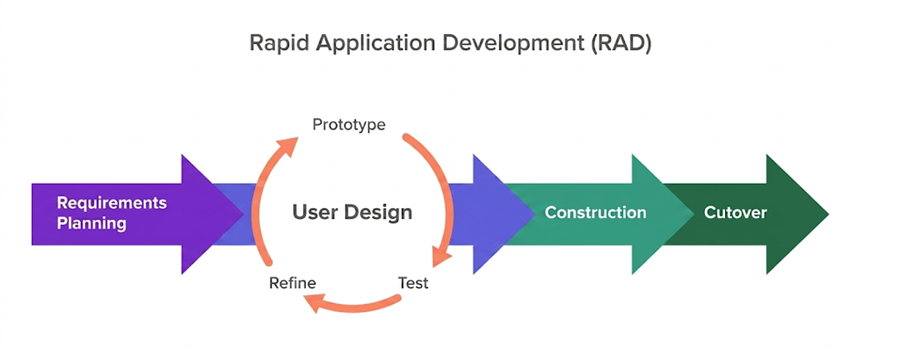
\includegraphics[width=0.99\textwidth]{image.png}
    \caption{Rapid Application Development (RAD) Model}
    \label{fig:placeholder}
\end{figure}
\hspace*{2em} RAD is a software development methodology emphasizing flexibility, speed, and user involvement. Its phases encompass requirements planning, user design, construction, and cutover. This approach enables rapid and adaptive system development through iterative cycles and prototyping [16]. The WeldTrack Inventory Management System with Cost Tracking for Gobole’s Welding Shop. Through the design, construction, and evaluation of a system goal at addressing practical issues such as inventory inaccuracy and inadequate project costing. It is descriptive in that it analyzes the shop’s current methods for material management, stock monitoring, and job order cost tracking. By thoroughly understanding these existing workflows and challenges, the system can be customized to fit the shop’s specific needs. Together, these two approaches ensure that the resulting solution is both practical and closely adapted to the shop’s operational environment.


 \subsection*{Requirements Planning}
\hspace*{2em} The proponents collaborate with the shop owner and staff to define booking, assigned-work, stock tracking, low-stock alert, project-cost, and reporting requirements.

 \subsection*{User Design}
\hspace*{2em} Through a series of workshops, users interact with initial prototypes of WeldTrack. The proponents present wireframes and mockups of key modules like inventory dashboards, job order forms, and material issuance interfaces. User feedback on layout, terminology, and workflow is immediately incorporated, ensuring the system's design aligns with shop floor expectations before any heavy coding begins.

 \subsection*{Prototype}
\hspace*{2em} The team develops a working, high-fidelity version of WeldTrack based on the approved user design. This prototype includes interactive but limited versions of essential features such as inventory tracking, job order creation, and material issuance allowing users to click through screens, input test data, and experience the core workflow. Unlike a static mockup, this prototype provides a tangible model ready for immediate testing, though it is not a fully functional production system. The process is iterative, with each major module inventory, costing, appointments, quotations, and reporting being prototyped individually.

 \subsection*{Test}
\hspace*{2em} The prototype undergoes structured testing by both the development team and a small group of end-users, including shop staff and a manager. The testing focuses on three main areas: functional testing verifying that features work as intended, usability testing ensuring users can navigate the prototype without confusion and that buttons and labels are natural, and workflow validation confirming that the prototype aligns with the actual shop floor process for receiving materials, creating job orders, and tracking costs. Any defects, confusing elements, or missing requirements are recorded in a testing log.

 \subsection*{Refine}
\hspace*{2em} Using the documented results from the Test phase, the proponents systematically resolve each identified problem. Refinement activities include fixing functional bugs such as incorrect cost calculation logic, enhancing user interface elements moving a poorly placed button, incorporating missing features identified during testing like adding a confirmation dialog before material issuance, and modifying workflows to better reflect shop operations. Once refinements are complete, the updated prototype returns to the Prototype phase for further development, then moves back to Test. This iterative cycle—Prototype → Test → Refine → Prototype—continues until all requirements are met and users give their approval of the system.

 \subsection*{Construction}
\hspace*{2em} During iterative construction, users review booking approval, material issuance, estimated and actual labor calculation, final project costing, and reporting workflows. Feedback guides the next implementation cycle.

 \subsection*{Cutover}
 \hspace*{2em} This final phase covers system deployment, data migration from existing manual logs, end-user training, and formal go-live. The cutover includes rigorous acceptance testing to ensure all modules function correctly in the live environment. Post-deployment support and maintenance procedures are also established to handle future enhancements or bug fixes.

\subsection{System Requirements}
\hspace*{2em} The system requirements outline the necessary hardware, software, and operational requirements needed for the Weldtrack Inventory Management System with Cost Tracking to function properly. These are divided into requirements for the proponents during development and for the and user gobole’s welding shops staff management during deployment and access.

\begin{table}[h]
\centering
\caption{List of Hardware, Software, and Operational Requirements}
\begin{tabular}{p{5cm} p{4cm} p{5cm}}
\hline
\textbf{List of Computer Hardware} & \textbf{Minimum Requirements} & \textbf{Recommended Requirements} \\
\hline
Storage and Processor & 1.83 GHz dual-core, 15 GB available storage & 12th Gen Intel Core i3 or equivalent, 128 GB SSD or higher \\
\hline
\multicolumn{3}{l}{\textbf{List of Computer Software}} \\
\hline
Operating System & Windows 10 Pro 64-Bit & Windows 11 or Linux (Ubuntu 20.04+) \\
Web Browser & Google Chrome v. 120+ / Microsoft Edge v. 120+ & Latest version of any modern browser \\
Web Server & Uvicorn & Uvicorn with Python 3.12+ \\
\hline
\multicolumn{3}{l}{\textbf{List of Operation}} \\
\hline
Internet Connection & 25 Mbps & 50 Mbps or Higher \\
Laptop & Acer Aspire 3 15 & Acer Aspire 3 15 \\
\hline
\end{tabular}
\end{table}

 \subsection*{Technical Terms}
\hspace*{2em} Dashboard - The dashboard is the main graphical interface that users see upon logging into WeldTrack. It provides an at-a-glance overview of key metrics such as current stock levels, low-stock alerts, recent job orders, pending material issuances, and total inventory valuation. For managers, the dashboard includes summary charts and quick-access buttons to reports, enabling efficient monitoring of shop operations without navigating through multiple menus.
\hspace*{2em} Appointment Management - In the context of WeldTrack, appointment management refers to the scheduling and tracking of job orders or client service appointments at Gobole's Welding Shop. This feature allows staff to create, reschedule, or cancel job appointments, assign them to specific workstations or welders, and set statuses pending, in-progress, completed. It helps avoid double-booking and ensures that material reservations align with scheduled work, improving shop floor organization and customer service.
\hspace*{2em} Inventory Management covers current quantities, maintained unit prices, suppliers, material issuance, low-stock thresholds, and stock-movement history. Material issuance is linked to assigned bookings and tasks, and the backend rejects non-positive or insufficient quantities.
\hspace*{2em} Booking Management covers customer requests, administrator approval and scheduling, staff task assignment, labor and material recording, completion, and final project-price calculation. These are operational cost records rather than formal quotations or invoices.

\subsection{Conceptual Design and Architecture}
\hspace*{2em} Figure 1 presents the System Architecture for the proposed WeldTrack system. This architecture adopts a standard three‑tier design, separating the user interface presentation layer from the business logic application layer and data management data layer, thereby offering benefits in scalability, security, and maintainability.
\hspace*{2em} The Presentation Layer is a responsive Vue 3 and TypeScript application using Vite, Pinia, Axios, Tailwind CSS, and scoped custom styles. It provides separate customer, staff, and administrator dashboards on desktop and mobile browsers.
\hspace*{2em} The Application Layer uses Python and FastAPI. It authenticates HTTP-only cookie sessions, enforces Administrator, Staff, and Customer permissions, restricts customers to owned records and staff to assigned work, rejects insufficient inventory, and calculates estimated labor, actual labor, material, and final project costs.
\hspace*{2em} The Data Layer uses PostgreSQL 16 with SQLAlchemy and Alembic for relational records and MinIO for uploaded images. Database transactions and backend validation preserve consistent inventory and project-cost records.



\begin{landscape}
\subsection*{\textbf{System Architecture Design}}

\vspace*{\fill} 

\begin{center}
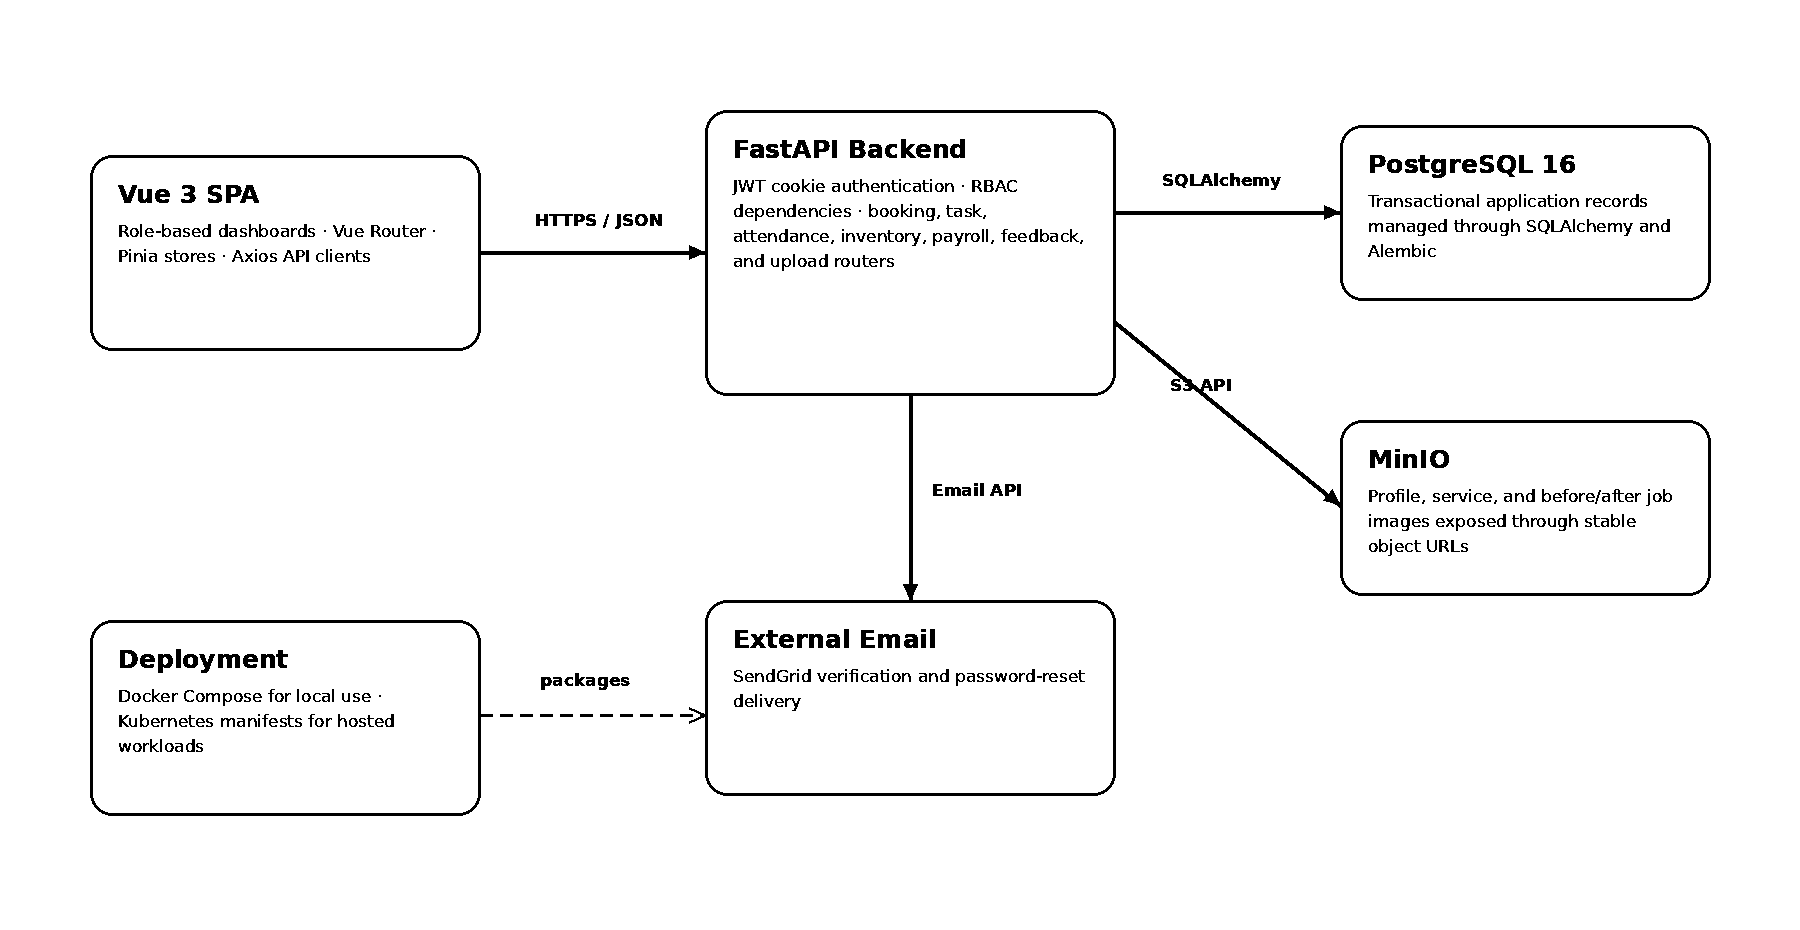
\includegraphics[width=0.99\linewidth]{weldtrack-architecture.png}  
\captionof{figure}{System Architecture Design}   
\label{fig:placeholder}
\end{center}

\vspace*{\fill} 

\end{landscape}

\newpage




% ------------------------------------------
% SECTION V
% ------------------------------------------

\subsubsection{User Case Diagram}
\hspace*{2em} Annex C.1 presents the three application actors. Customers manage addresses, create and track their own bookings, and provide feedback. Staff record attendance, view assigned tasks, submit project images and material usage, and access their own payslips and contributions. Administrators approve and schedule bookings, assign tasks, manage inventory, services, users and payroll, complete project costing, generate reports, and moderate feedback.

\subsection{Project Schedule and Management}
\hspace*{2em} A project timeline presents a sequence of events, offering the team a quick overview of their tasks. Both a schedule and a timeline serve as essential tools for planning and tracking progress: the schedule breaks down specific tasks and activities, while the timeline indicates anticipated start and end dates. Used together, they help maintain organization and ensure the project stays on course

\subsubsection{Work Breakdown Structure}
\hspace*{2em} The Work Breakdown Structure see Annex A.1 organizes all small tasks needed to accomplish the project. It breaks the work into smaller pieces so the team can plan, schedule, and track progress. Each task has an ID, duration, and predecessor dependencies

\subsubsection{Gantt Chart}
\hspace*{2em} The Gantt chart see Annex A.2 shows the timeline for developing WeldTrack. It visually displays tasks, start and end dates, dependencies, and progress. The project spans 16 weeks one semester. Milestones include: Requirements Approved end week 2, Prototype Validated end week 5, Alpha Release end week 8, Beta Release end week 12, UAT Complete end week 14, Final Deployment end week 16.
\subsection{Testing and Evaluation}
\hspace*{2em} The system’s quality and functionality will be verified through a structured testing process that combines iterative prototyping with hands on reviews by the evaluation panel. Starting with an initial prototype, the development will go through three rounds of prototyping. After each round, the panel shop owner, staff, and IT experts meets to review the system against required features, ease of use,and performance.
\hspace*{2em} Their feedback guides improvements. Alongside these manual reviews, each prototype undergoes functional testing all features work correctly, usability testing smooth interaction, and compatibility testing different devices and browsers. The third prototype will undergo acceptance testing, where the panel checks reliability, speed, and user satisfaction. Only when all issues are fixed and the panel gives formal approval will the system be considered validated.

\subsubsection{Evaluation Instrument}
\hspace*{2em} The assessment tool is a User Acceptance Testing questionnaire based on ISO/IEC 25010:2023 and consistently evaluates Functional Suitability, Performance Efficiency, and Interaction Capability.

\subsubsection{Respondents of the Study}
\hspace*{2em} The evaluation will involve 15 respondents selected through purposive sampling, representing the primary user groups of Gobole's Welding Shop. The owner or administrator evaluates functional suitability of management features and overall system performance; managers focus on inventory control, job order management, and cost tracking; staff assess the usability, speed, and reliability of daily operations; and IT experts evaluate technical aspects such as functional completeness and performance optimization. 

\begin{table}[h]
\centering
\caption{Respondents}
\begin{tabular}{p{6cm} p{6cm}}
\toprule
\textbf{Respondents Category} & \textbf{Numbers of Evaluators} \\
\midrule
Shop Owner / Administrator & 1 \\
Shop Manager / Supervisor & 2 \\
Shop Floor Staff  & 8\\
IT Experts (Faculty / External) &  4\\
Total & 15 \\
\bottomrule
\end{tabular}
\end{table}

\subsubsection{Statistical Treatment of Data}
\hspace*{2em} To interpret the UAT results, the proponents will use descriptive statistics, with the weighted mean as the main statistical tool. The evaluation instrument contains 16 statements based on the ISO/IEC 25010 characteristics (10 for Functional Suitability, 6 for Performance Efficiency), each rated on a 5 point Likert scale. Responses from 15 evaluators will be quantified and interpreted to assess overall acceptability.

\begin{table}[h]
\centering
\caption{Likert Scale Interpretation}
\begin{tabular}{p{3cm} p{4cm} p{4cm}}
\toprule
\textbf{Rating} & \textbf{Mean Range} & \textbf{Interpretation} \\
\midrule
5 & 4.50 – 5.00 & Excellent \\
4 & 3.50 – 4.49 & Good \\
3 & 2.50 – 3.49 & Fair\\
2 & 1.50 – 2.49 & Poor \\
1 & 1.00 – 1.49 & Very Poor \\
\bottomrule
\end{tabular}
\end{table}

\newpage
\bibliographystyle{plain}
\begin{thebibliography}{9}  

\bibitem{ref1}
Dynamics Square USA, "How Dynamics 365 Transforms MIG, TIG, and                 Fabrication Shops," MSDynamicsWorld.com, June 13, 2025, [Online]. Available: https://msdynamicsworld.com

\bibitem{ref2}
N. V. Huan, N. T. Hang, and N. T. Hue, "A digital transformation approach from traditional to virtual practice: A case study of gas welding corner-welding," VMOST Journal, 2025, Doi: 10.31276/VMOSTJOSSH.2024.0081.,
\emph{VMOST Journal}, 2025, Doi: 10.31276/VMOSTJOSSH.2024.0081.

\bibitem{ref3}
J. L. A. Baylosis, B. J. A. Abiles, M. L. P. Catungal, and P. C. Encarnacion, “Web-based Inventory Management System,” International Journal, vol. 12, no. 5, 2023.

\bibitem{ref4}
W. Aribowo Probonegoro and L. Indah Sari, "Web-Based Material Inventory Information System for ALAR Welding Workshop," International Journal of Information System and Technology (IJISTECH), vol. 9, no. 1, pp. 73-81, 2025.

\bibitem{ref5}
S. Singh, R. Kumar, A. Badhoutiya, U. Sharma, A. Alkhayyat, and S. K. Shah, "Web-Based Inventory, Stock Monitoring and Control System Powered by Local Encrypted Web Server," 2024 11th International Conference on Computing for Sustainable Global Development (INDIACom), 2024, pp. 741–744.

\bibitem{ref6}
A. Yoraeni, A. Margaret, M. Ifadah, and A. Mulyono, “Implementation of a Web-Based Inventory Management Information System,” bit-Tech, vol. 8, no. 2, pp. 2338–2347, Dec. 2025, doi: 10.32877/bt.v8i2.3245.

\bibitem{ref7}
M. K. Alam, O. A. Thakur, and F. T. Islam, “Inventory management systems of small and medium enterprises in Bangladesh,” Journal of Small Business and Enterprise Development, vol. 30, no. 1, pp. 8–18, 2023. doi: 10.1108/JSBED-01-2022-0021.

\bibitem{ref8}
R. Bose, H. Mondal, I. Sarkar, and S. Roy, “Design of smart inventory management system for construction sector based on IoT and cloud computing,” e-Prime – Advances in Electrical Engineering, Electronics and Energy, vol. 2, p. 100051, 2022. doi: 10.1016/j.prime.2022.100051.

\bibitem{ref9}
B. Odasco and M. Saong, “Analysis of the Inventory Management System        Towards Enhanced University Service Delivery,” IJSTEM, vol. 3, no. 3, pp. 103–132, Sep. 2023, doi: 10.53378/353010

\bibitem{ref10}
J. M. D. Jesalva, A. E. M. Mesia, K. M. W. Pangan, G. S. Trillana, R. B. Avila, E. F. Dayao, and J. D. Espino, "A Web-Based Inventory Management System for The Properties and Supplies Office," Int. J. Acad. Multidiscip. Res., vol. 8, no. 7, pp. 484–488, Jul. 2024.

\bibitem{ref11}
A. K. Laping, C. A. Mendoza, K. N. Tiulentino, R. M. Villaraza, G. C. Bucu, and J. K. Ngo, "Designing an Inventory Management System for Convenience Store X Using Design Thinking Approach," in Proc. Int. Conf. Industrial Engineering and Operations Management, De La Salle University, Manila, Philippines, 2023, pp. 1703–1715.

\bibitem{ref12}
M. T. Tanaman, J. L. A. Baylosis, B. J. A. Abiles, M. [7] L. P. Catungal, and P. C. Encarnacion, “Web-based Inventory Management System,” International Journal of Science and Applied Information Technology, vol. 12, no. 5, pp. 1–5, Oct. 2023. doi: 10.30534/ijsait/2023/021252023.

\bibitem{ref13}
C. M. M. Cabantog, V. C. D. V. Dizon, D. V. Intacto, and E. J. D. G. Magpayo, “Inventory management system of the selected pharmacies in the City of Baliwag: An assessment,” unpublished undergraduate research, Baliuag Univ., Baliwag, Philippines, 2026.

\bibitem{ref14}
D. Novitasari and A. H. Wijaya, "Web Based Ordering and Inventory Information System for Online Printing Services with TAM Method," Journal Tech-E, vol. 5. no. 1, 2021

\bibitem{ref15}
Republic Act No. 10173, An Act Protecting Individual Personal Information in Information and Communications Systems in the Government and the Private Sector, Creating for this Purpose a National Privacy Commission, and for Other Purposes, (August 15, 2012).

\bibitem{ref16}
M. W. Tjia, David, and J. Hendrik, “Web-Based Inventory System Design Using Rapid Application Development Method at PT. ALFA SCORPII,” vol. 4, no. 3, pp. 1–6, Jun. 2025, e-ISSN: 2808-4519.

\end{thebibliography}
\clearpage
\thispagestyle{empty}   
\null\vfill
\begin{center}
\Huge Annexes
\end{center}
\vfill
\clearpage

\subsection*{Annex A - Project Schedule and Work Breakdown Structure}
\hspace*{2em}This section contains the Work Breakdown Structure (WBS) and the Gantt Chart, detailing the timeline, milestones, and task allocations for the entire capstone project lifecycle.	 
\clearpage
\subsection*{A.1 Work Breakdown Structure (WBS)}


\begin{table}[h]
\centering

\begin{tabular}{p{2cm} p{6cm} p{2cm} p{2cm}}
\toprule
\textbf{Task ID} & \textbf{Task Description} & \textbf{Duration} & \textbf{Predecessor} \\
\midrule
Requirements Planning& &  &  \\
1 & Identify client & 4d & T1 \\
2 & Identify specific pain points& 5d &T2 \\
3 & Define project scope & 7d & T3 \\
4 & Define system boundaries and limitations & 3d & T4 \\
5 & Document requirements  & 13d & T5 \\
User Design &&& \\
6& Create UML diagrams& 10d & T6 \\
7&Create wireframes and mockups & 15d & T7\\
8&Conduct usability testing & 9d & T8\\
9&Design validation and redesign&13d& T9\\
Construction&&& \\
10 &Develop frontend &76d& T10 \\
11 &Develop inventory tracking &9d & T11 \\
12 &Develop project-cost calculation& 10d & T12 \\
13 &Develop appointment scheduling &10d & T13 \\
14 &System testing and debugging &25d & T14 \\
Cutover &&&\\
15 &Plan development &2d & T15\\
16 &Deployment system on cloud hosting&15d &T16\\
17 &Conduct system evaluation &12d & T17\\
18 &conduct user training &12d &T18 \\

\bottomrule
\end{tabular}
\end{table}


\begin{landscape}

\subsection*{A.2 Gantt Chart}
\vspace*{\fill} 

\begin{center}
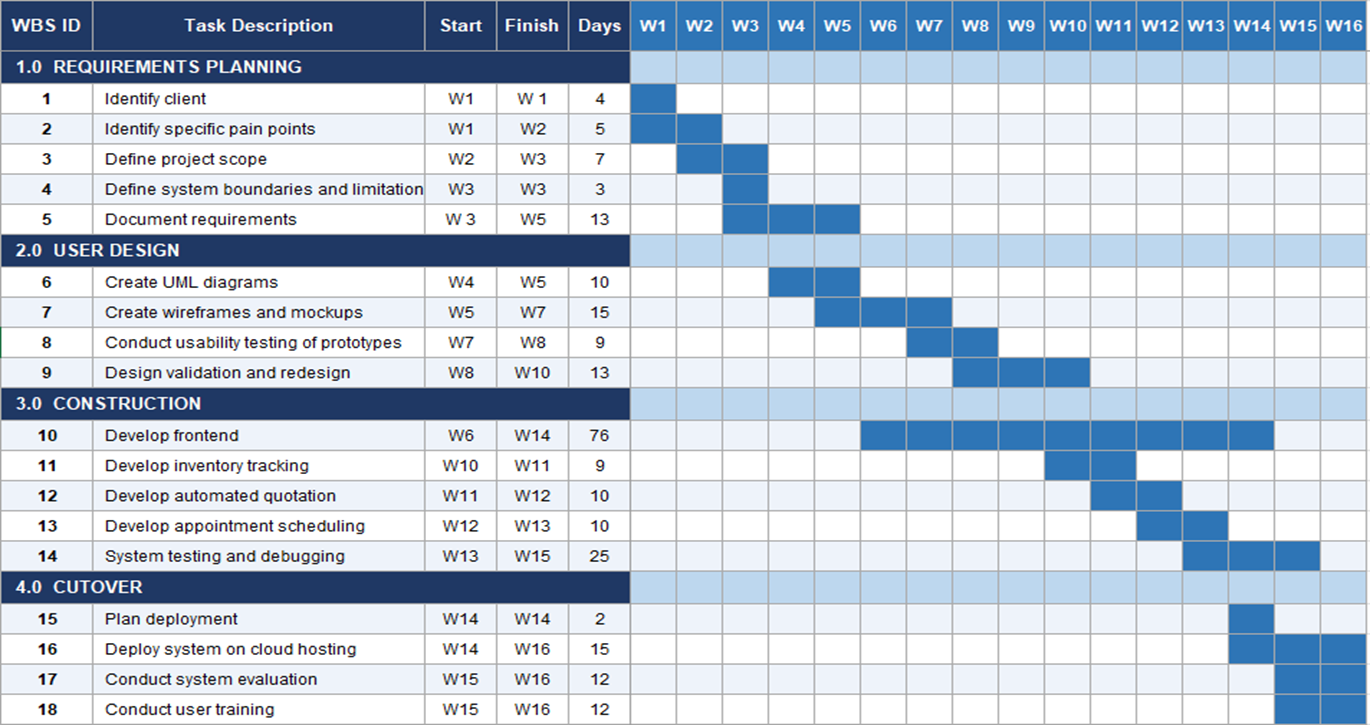
\includegraphics[width=1.05\linewidth]{century/gantt.png}
\captionof{figure}{Project Gantt Chart}
\label{fig:placeholder}

\end{center}
\vspace*{\fill} 

\end{landscape}






\subsection*{Annex B - Software Requirements Specification (SRS)}

\hspace*{2em} This document outlines every requirement that the WeldTrack system must meet, organized into functional requirements and non‑functional requirements These requirements are directly based on the manual inventory and costing challenges faced by Gobole’s Welding Shop. The Software Requirements Specification (SRS) also includes definitions, user classes, and user stories to ensure that developers, testers, and shop stakeholders share a clear, consistent understanding of the system’s scope and quality objectives.
\hspace*{2em} WeldTrack covers customer booking, administrative scheduling, assigned staff work, inventory monitoring, estimated and actual project costing, completed-project revenue, attendance, payroll, feedback, and operational reporting.

\newpage

\subsection*{Definitions and Abbreviations}


\begin{table}[h]
\centering

\begin{tabular}{p{6cm} p{6cm}}
\toprule
\textbf{Term / Acronym} & \textbf{Definition} \\
\midrule
WeldTrack & Proposed web based inventory management system with cost tracking. \\
Job Order & Customer welding project requiring material issuance \\
RBAC & Role Based Access Control  \\
DPA &  Republic Act No. 10173 \\
ISO 25010 & International standard for software quality  \\
UAT & User Acceptance Testing \\
\bottomrule
\end{tabular}
\end{table}

\subsection*{User Classes and Characteristics}



\begin{table}[h]
\centering

\begin{tabular}{p{3cm} p{5cm} p{6cm}}
\toprule
\textbf{User Class} & \textbf{Technical Level} & \textbf{Description}  \\
\midrule
Customer & Low to moderate & Manages addresses, creates and tracks owned bookings, views costs, and provides feedback.\\
Staff Member & Low to moderate & Views assigned tasks, records attendance, labor, materials, and project images.\\
Admin / Shop Owner  & Moderate to high  & Manages users, services, bookings, assignments, inventory, payroll, reports, and final project costing. \\
IT Expert (Evaluator) &  High & Evaluates code modularity, database design, security compliance, maintainability. \\
\bottomrule
\end{tabular}
\end{table}


\newpage


\subsection*{B. 1 Functional Requirements}


\begin{table}[h]
\centering

\begin{tabular}{p{3cm} p{5cm} p{6cm}}
\toprule
\textbf{ID} & \textbf{Requirement} & \textbf{Description}  \\
\midrule
FR-01 & User authentication & Unique credentials; passwords hashed with bcrypt. \\
FR-02 & Role-based access & Three levels: Administrator, Staff, Customer, with ownership and assignment checks.\\
FR-03  & Booking Management  & Create, approve, schedule, track, complete, or cancel customer bookings. \\
FR-04 & Appointment scheduling & Administrator-approved project schedule dates. \\
FR-05&Inventory tracking&Current quantities, unit prices, suppliers, thresholds, and movements.\\
FR-06&Project-cost estimation&Calculates estimated labor cost from estimated hours and service hourly rate.\\
FR-07&Actual project costing&Calculates actual labor, material cost, final project price, and completed-project revenue.\\
FR-08&Reporting &Stock movement, financial, attendance, and completed-project summaries.\\
\bottomrule
\end{tabular}
\end{table}


\newpage


 \subsection*{B. 2 Non Functional Requirements}


\begin{table}[h]
\centering

\begin{tabular}{p{3cm} p{5cm} p{6cm}}
\toprule
\textbf{ID} & \textbf{Characteristic} & \textbf{Requirement}  \\
\midrule
NFR-01 & Functional Suitability & Supports documented booking, inventory, task, costing, attendance, payroll, and reporting workflows. \\
NFR-02 & Reliability & PostgreSQL transactions and backend validation preserve consistent records.\\
NFR-03  & Usability  & Responsive Vue 3 and Tailwind CSS interface with clear validation feedback. \\
NFR-04 &  Performance Efficiency & Response ≤3 seconds under normal network conditions.\\
NFR-05&Security&HTTP-only cookie authentication, password hashing, RBAC, ownership checks, and assignment checks.\\
NFR-06&Maintainability&Modular Vue/TypeScript and FastAPI/SQLAlchemy code with Alembic migrations.\\
NFR-07& Compatibility &Responsive on desktops, tablets, Chrome, Edge.\\

\bottomrule
\end{tabular}
\end{table}


\clearpage

\subsection*{B. 3 User Stories}


\begin{table}[h]
\centering

\begin{tabular}{p{3cm} p{5cm} p{6cm}}
\toprule
\textbf{ID} & \textbf{User Story} & \textbf{Acceptance Criteria}  \\
\midrule
US-01 & As staff, I want to view real time stock so I can check availability quickly & Stock list shows current quantities; low stock items highlighted. \\
US-02 & As staff, I want to issue materials to a job order so inventory is reduced and cost tracked.& Release checks stock, deducts quantity, records against job order. \\
US-03  & As administrator, I want to approve bookings, record estimated labor hours, and assign staff. & Only authorized administrators can approve and assign work. \\
US-04 & As assigned staff, I want to record actual hours and materials. & The backend calculates actual labor and rejects insufficient inventory.\\
US-05&As owner, I want a final project price based on persisted work records.& Backend total equals actual labor cost plus recorded material cost. \\

\bottomrule
\end{tabular}
\end{table}


\newpage

\subsection*{Annex C - UML Diagrams}
\hspace*{2em }This annex provides a comprehensive visual representation of the sys
tem’s architecture and workflow through the Unified Modeling Language 
(UML).
\newpage
\subsection*{C.1 Use Case Diagram}
\vspace*{\fill}

\begin{center}
\centering
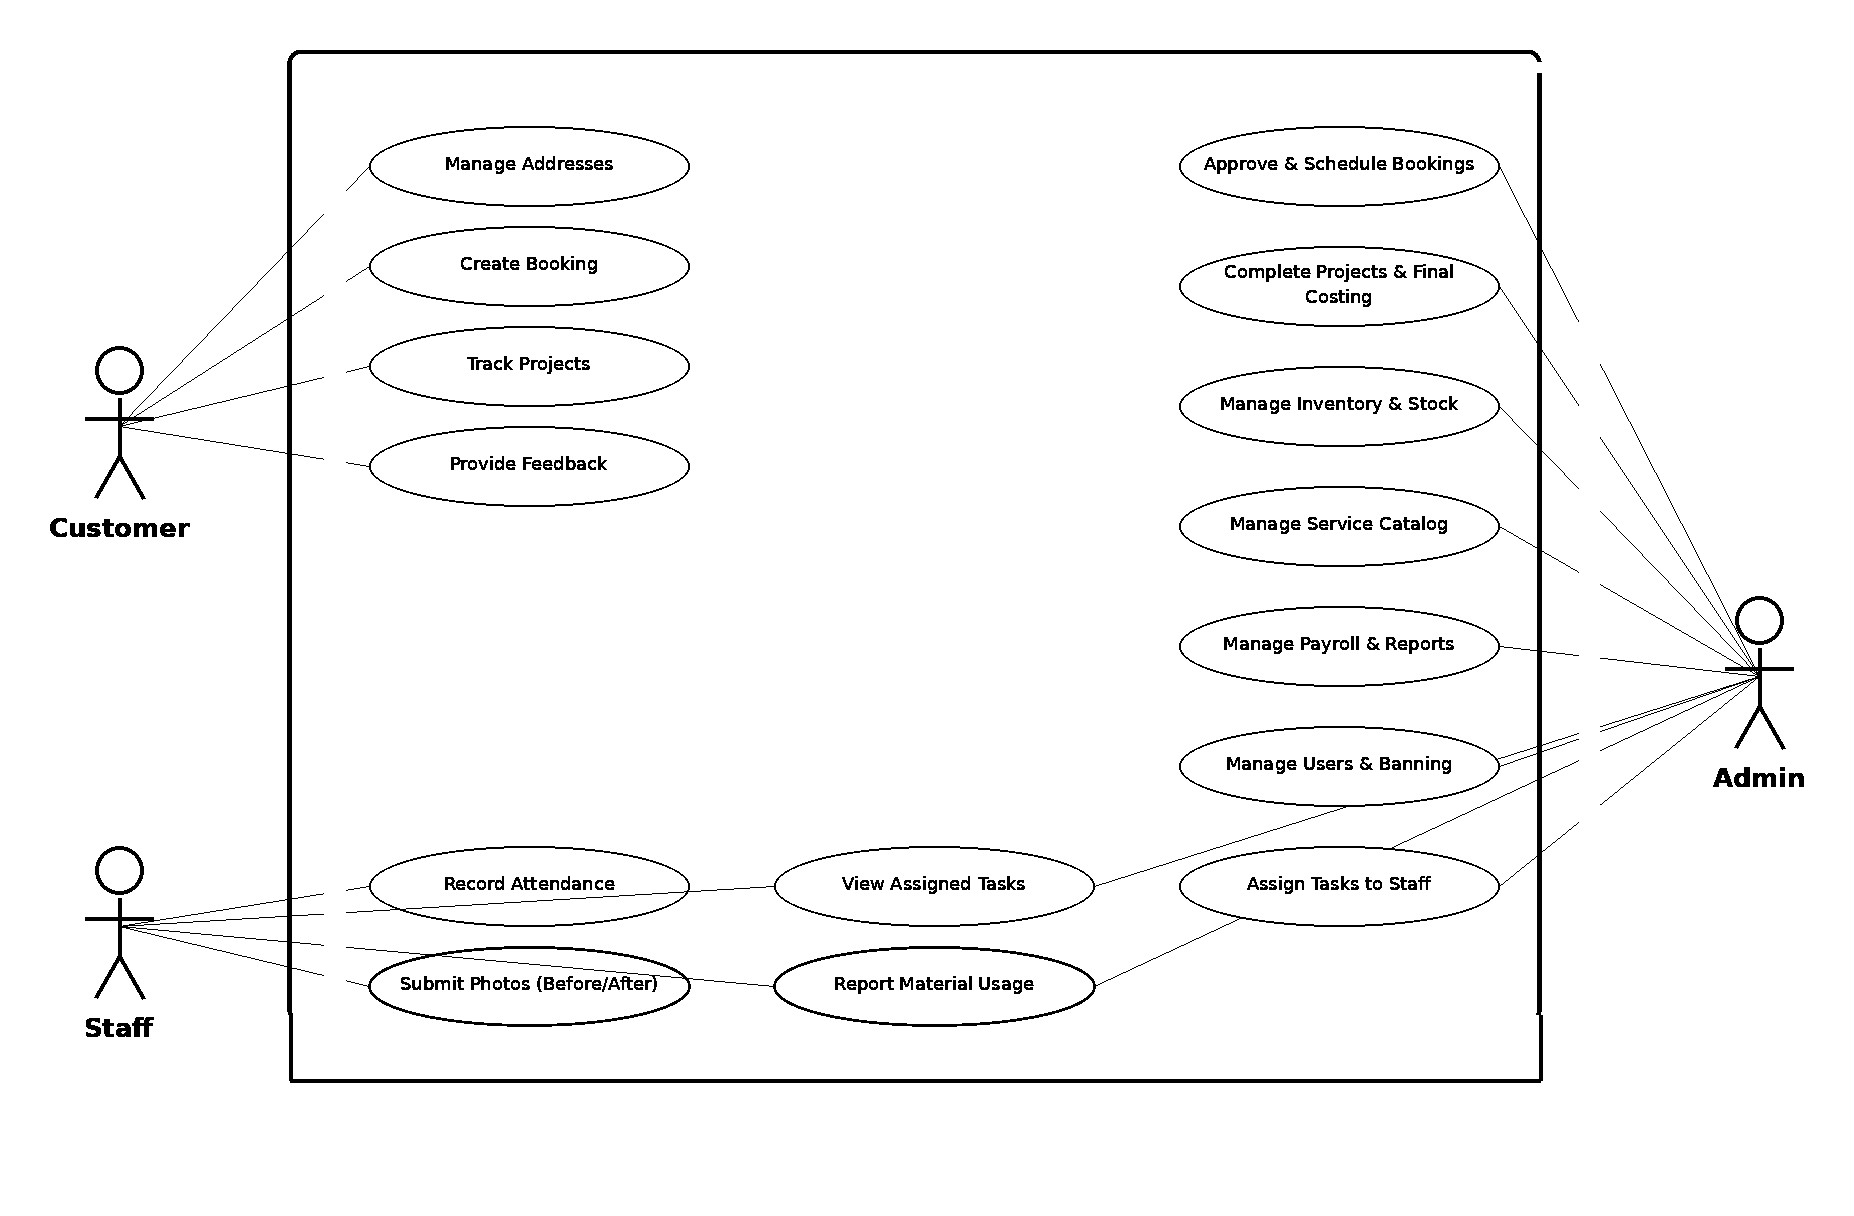
\includegraphics[width=1.0\linewidth]{weldtrack-use-case.png}
\label{fig:placeholder}
\vspace*{\fill}

\end{center}

\subsection*{C.2 Activity Diagrams}
\vspace*{\fill}

\begin{center}
\centering
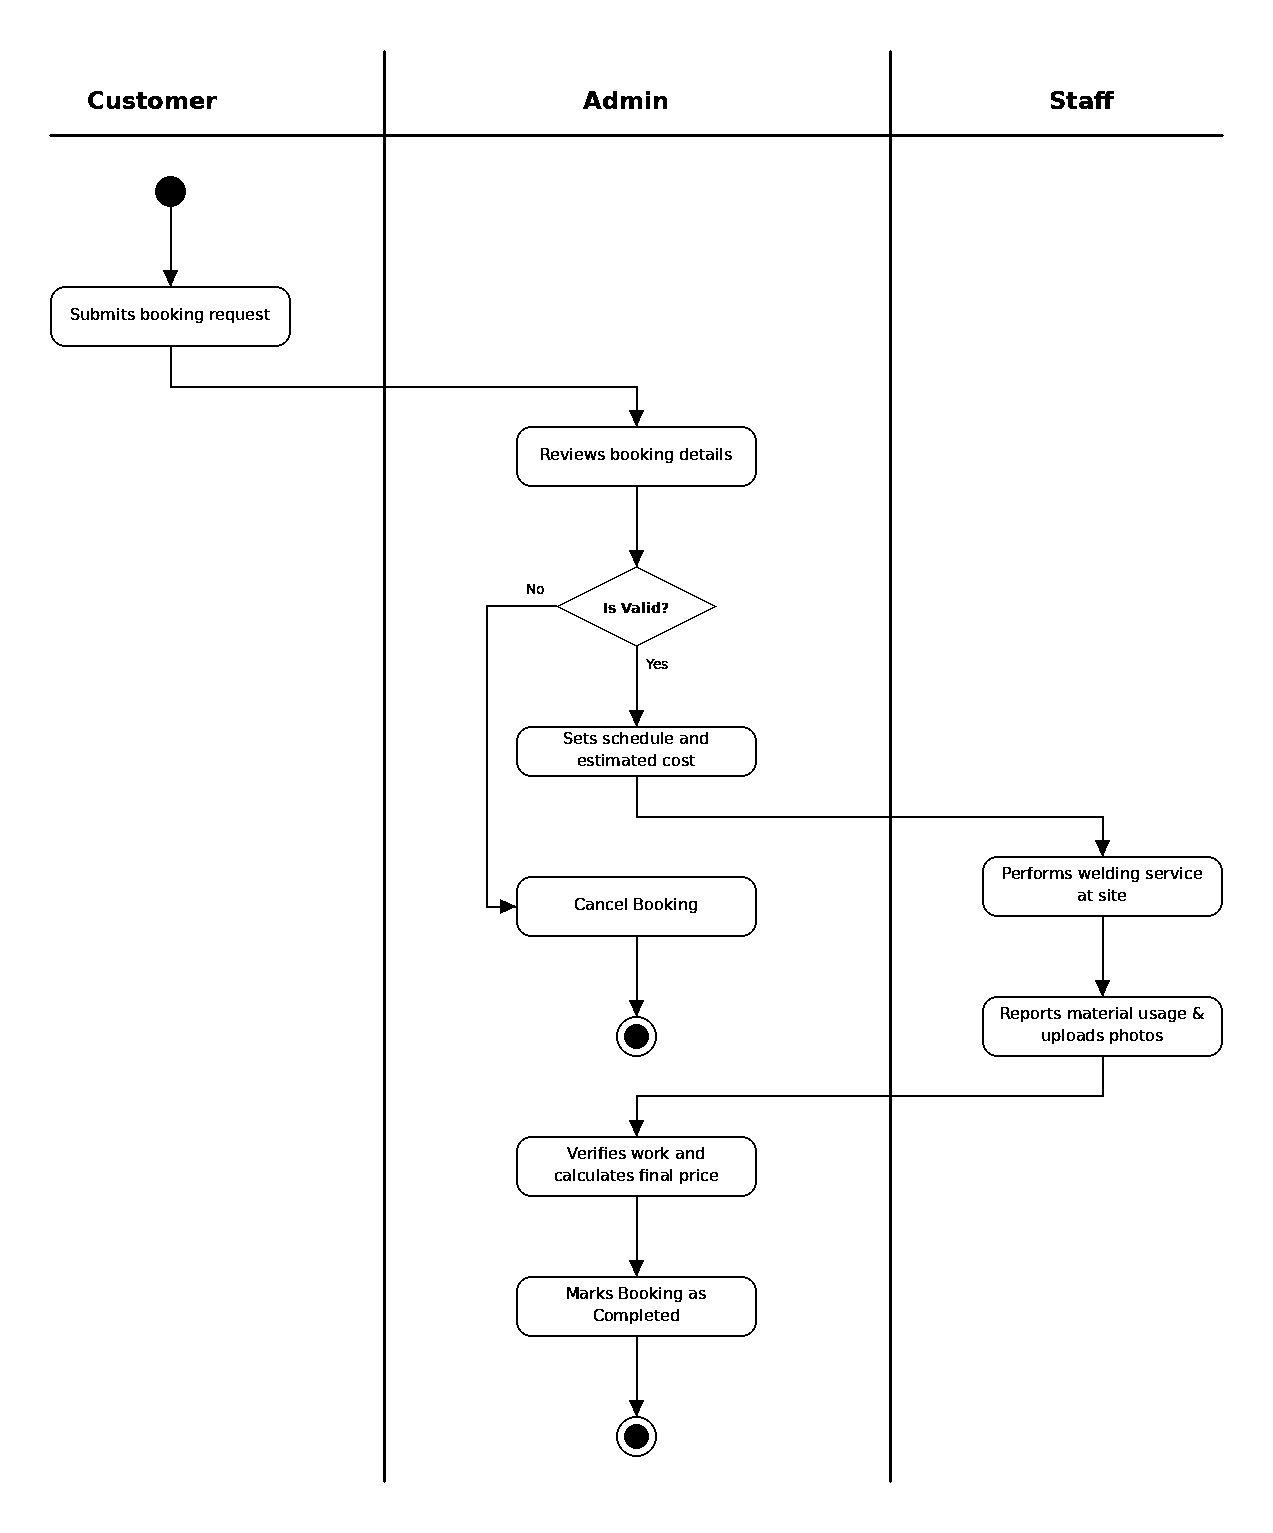
\includegraphics[width=0.85\linewidth]{weldtrack-activity.png}
\end{center}

\clearpage

\newpage

\subsection*{C.3 Sequence Diagrams}
\vspace*{\fill}

\begin{center}
\centering
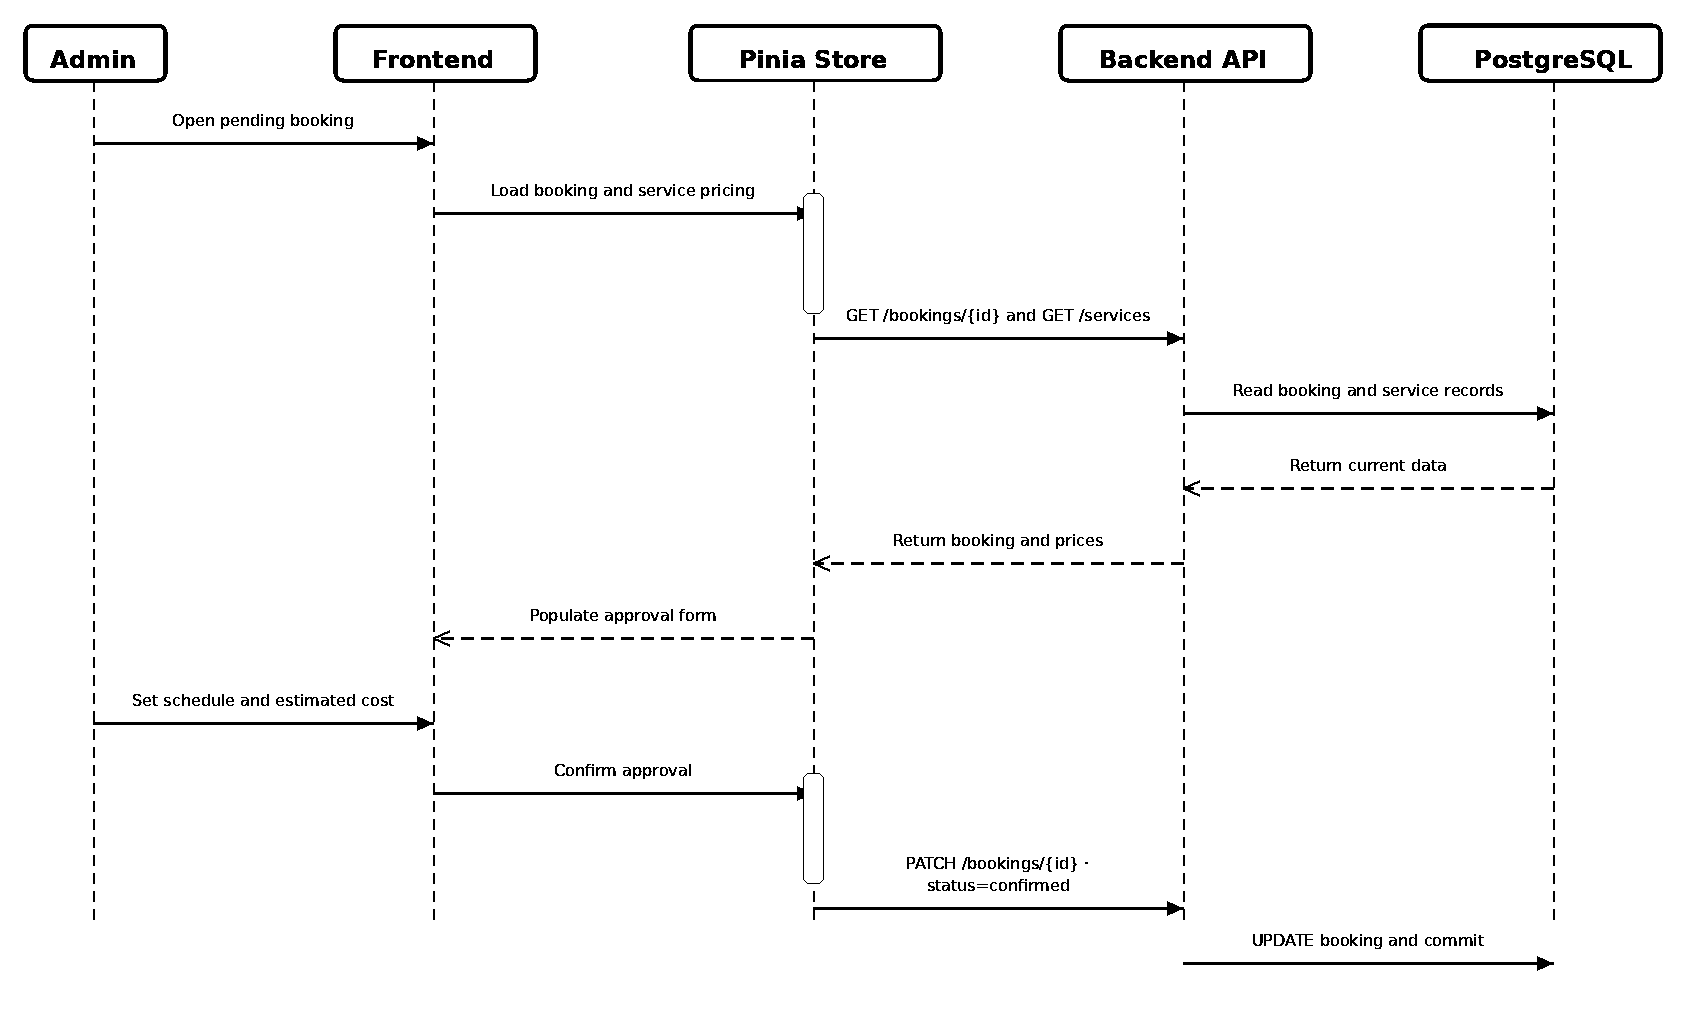
\includegraphics[width=1\linewidth]{weldtrack-sequence.png}
\vspace*{\fill}
\end{center}

\clearpage

\newpage

\subsection*{C.4 Entity Relationship Diagram (ERD)}
\vspace*{\fill}
\begin{figure}
\centering
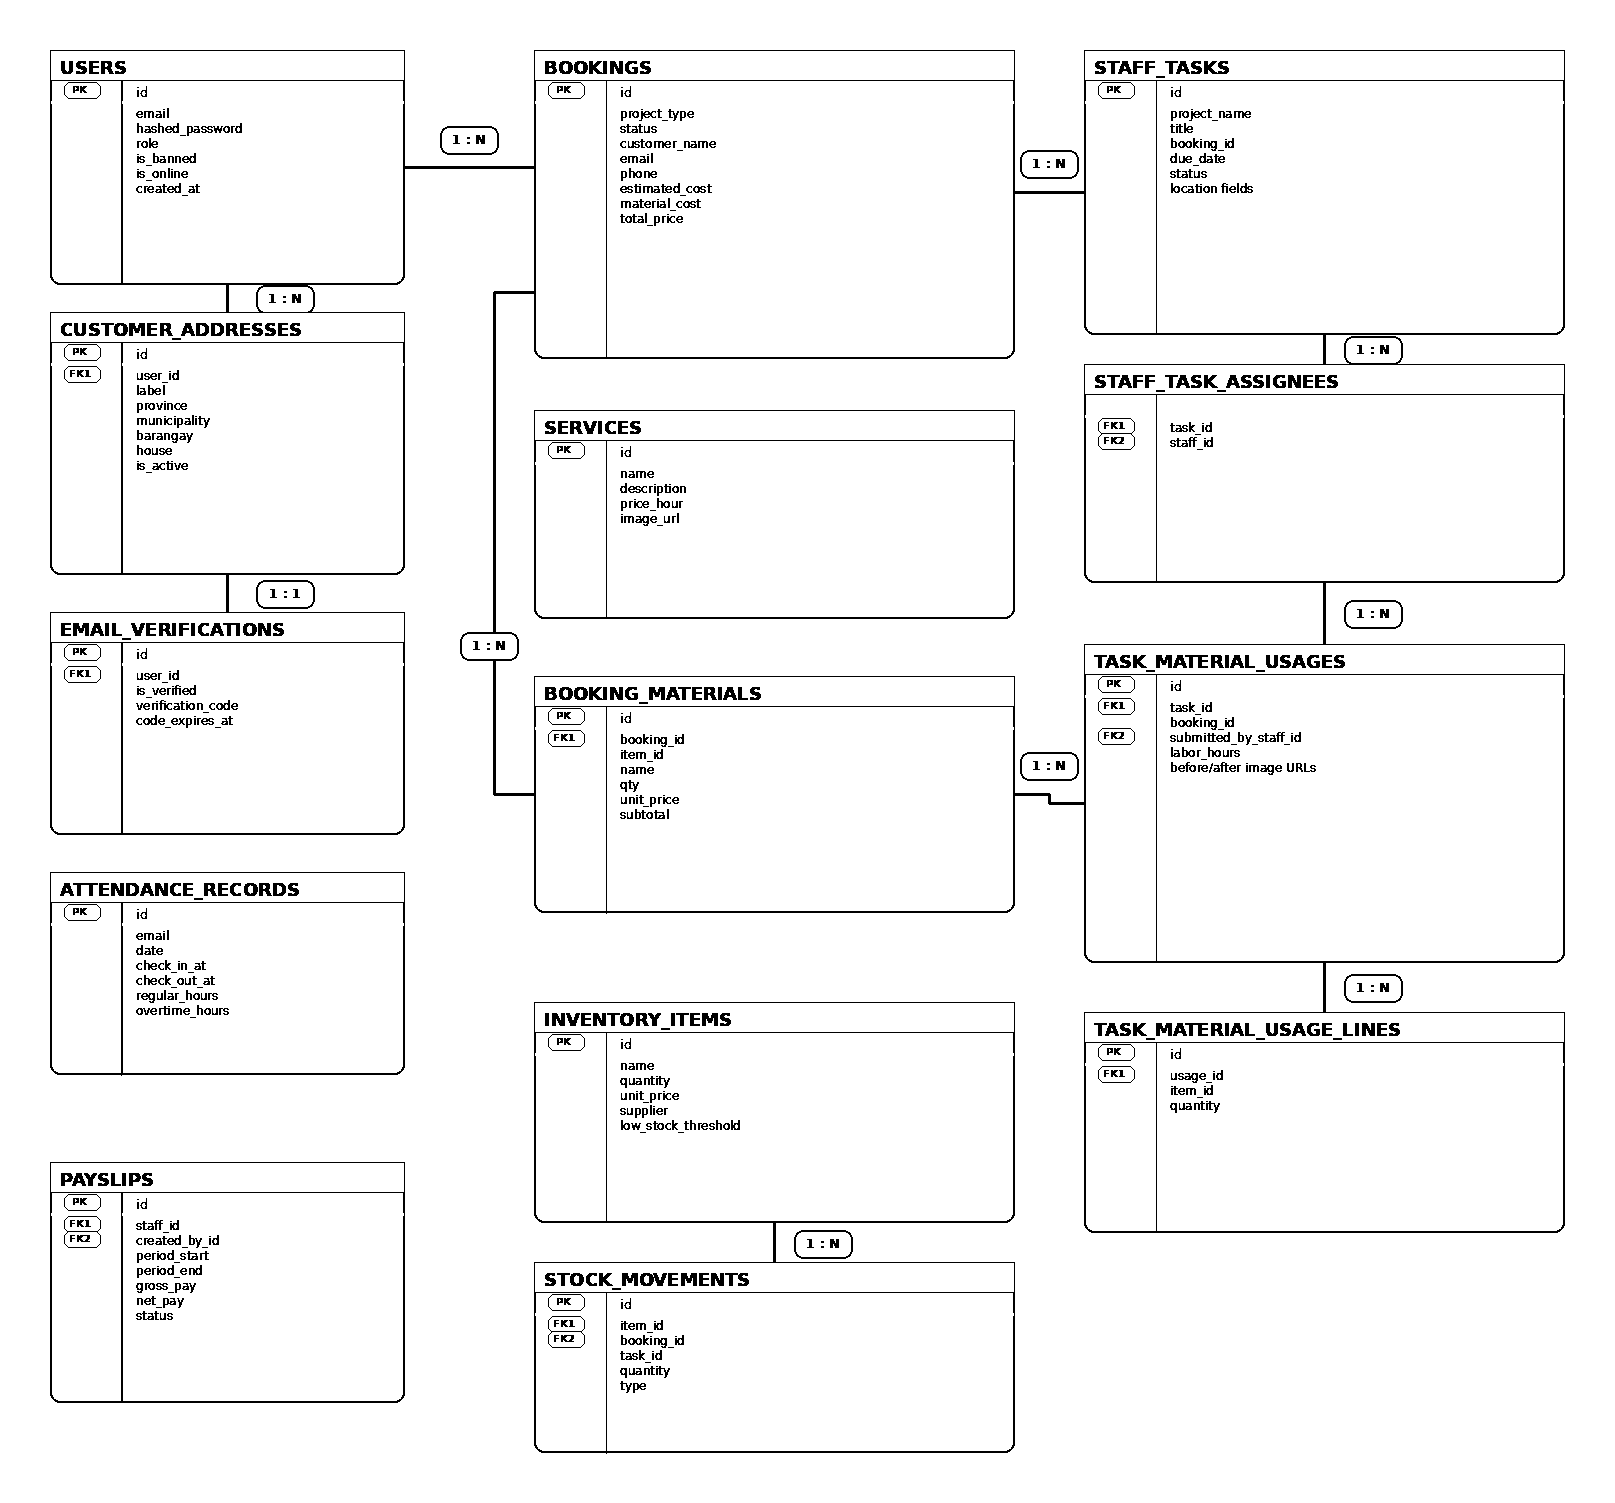
\includegraphics[width=1\linewidth]{weldtrack-erd.png}
\label{fig:placeholder}
\vspace*{\fill}
\end{figure}


\clearpage

\newpage

\subsection*{Annex D - System Test Cases and Performance Reports}
\hspace*{2em} This annex defines test cases for authentication, record-level authorization, booking ownership, assigned tasks, insufficient-stock prevention, low-stock alerts, estimated and actual labor costing, recorded material cost, backend final-price calculation, and reporting. Actual results and status must be completed only after each test is executed.


\newpage

\begin{landscape}


\begin{center}\textbf{Inventory Management}\end{center}
\centering


\begin{tabular}{p{2cm} p{4cm} p{5cm} p{5cm} p{3cm} p{2cm}}
\toprule
\textbf{Test ID} & \textbf{Pre-Condition} & \textbf{Test Steps} & \textbf{Expected Result} & \textbf{Actual Result} & \textbf{Status} \\
\midrule
TC-001 & Staff logged in, no existing stock of “Welding Rod 3.2mm” & 1. Navigate to Purchase Receiving.
2. Enter: 50 units @ ₱120/unit.
3. Submit receipt.
 & Stock = 50 units and maintained unit price = PHP 120.00. Item recorded. & & Pending\\
TC-002&Existing stock: 50 units @ ₱120.00.& 1. Receive additional 30 units @ ₱140.00.
2. Save item. & Maintained quantity and unit price are saved and displayed accurately. & & Pending\\
TC-003 & Stock of “Flap Disc” = 10 units. & 1. Issue 15 units to a job order.
2. Click “Issue”. & System rejects issuance, shows “Insufficient stock (10 available)”, no deduction made. & & Pending\\
TC-004&  Stock of “Metal Sheet” = 20 units. & 1. Issue 5 units to job order 
2. Immediately view inventory list &Stock updates to 15 units without page refresh (AJAX/WebSocket).& & Pending\\


\bottomrule
\end{tabular}


 


\end{landscape}


\clearpage

\newpage


\begin{landscape}


\begin{center}\textbf{Job Order}\end{center}
\centering

\begin{tabular}{p{2cm} p{4cm} p{5cm} p{5cm} p{3cm} p{2cm}}
\toprule
\textbf{Test ID} & \textbf{Pre-Condition} & \textbf{Test Steps} & \textbf{Expected Result} & \textbf{Actual Result} & \textbf{Status} \\
\midrule
TC-005 & Manager logged in, materials exist with cost. & 1. Create TC-005 for “Gate Fabrication”.
2. Issue 10 units of “Angle Bar” (avg cost ₱200).
3. View job order cost summary.
 & TC 002 shows material cost = ₱2,000. Total project cost calculated (materials + optional labor). & & Pending\\
TC-006&Staff tries to issue materials without selecting a job order.& 1. Click “Issue Materials”.
2. Leave job order field blank.
3. Submit.
 &System shows “Please select a valid job order” and blocks issuance. & & Pending\\

\bottomrule
\end{tabular}

    
\end{landscape}

\clearpage

\newpage


\begin{landscape}

    

\begin{center}\textbf{Low Stock Alert}\end{center}
\centering

\begin{tabular}{p{2cm} p{4cm} p{5cm} p{5cm} p{3cm} p{2cm}}
\toprule
\textbf{Test ID} & \textbf{Pre-Condition} & \textbf{Test Steps} & \textbf{Expected Result} & \textbf{Actual Result} & \textbf{Status} \\
\midrule
TC-007 & Reorder threshold for “Grinding Disc” = 20 units. Current stock = 22 units.
 & 1. Issue 5 units to a job order. 2. View dashboard.
 & Stock = 17 units (<20). Dashboard shows red alert badge and “Low stock: Grinding Disc”. & & Pending\\
TC-008 &Admin logged in. & 1. Edit “Welding Rod 3.2mm”.
2. Set reorder point = 100 units.
3. Save.

 &Threshold saved. When stock falls below 100, alert triggers. & & Pending\\

\bottomrule
\end{tabular}


\end{landscape}

\clearpage

\newpage


\begin{landscape}

    

\begin{center}\textbf{Appointment and Schedule Management}\end{center}
\centering

\begin{tabular}{p{2cm} p{4cm} p{5cm} p{5cm} p{3cm} p{2cm}}
\toprule
\textbf{Test ID} & \textbf{Pre-Condition} & \textbf{Test Steps} & \textbf{Expected Result} & \textbf{Actual Result} & \textbf{Status} \\
\midrule
TC-009 & Manager has a confirmed job order TC-005
 & 1. Open appointment calendar.
2. Select date/time (e.g., Apr 25, 9:00 AM).
3. Assign to welder “John”.
4. Save.
 & Appointment saved, appears on calendar. No double booking for that time slot. & & Pending\\
TC-010 &Existing appointment: Apr 25, 9:00 AM – Welder John. & 1. Try to schedule another job with Welder John on same date/time.
2. Submit.
 &System shows “Time slot already booked” and prevents save. & & Pending\\

\bottomrule
\end{tabular}


\end{landscape}

\clearpage

\newpage


\begin{landscape}

    

\begin{center}\textbf{Reporting}\end{center}
\centering

\begin{tabular}{p{2cm} p{4cm} p{5cm} p{5cm} p{3cm} p{2cm}}
\toprule
\textbf{Test ID} & \textbf{Pre-Condition} & \textbf{Test Steps} & \textbf{Expected Result} & \textbf{Actual Result} & \textbf{Status} \\
\midrule
TC-011 & Multiple materials with maintained quantities and unit prices.
 & 1. Navigate to Reports → Inventory Valuation.
2. Set date range (current month).
3. Generate.
 & Report shows each material: quantity, avg cost, total value. Totals match manual calculation. & & Pending\\
TC-012 &TC 006 has material issuances logged. & 1. Go to Reports → Job Order Cost.
2. Select TC 006
3. Generate PDF.
 &PDF includes: issued materials, quantities, unit cost (weighted avg), subtotal, and grand total.\\

\bottomrule
\end{tabular}


\end{landscape}

\clearpage

\newpage


\begin{landscape}

    

\begin{center}\textbf{Role-Based Access Control (RBAC) and Security}\end{center}
\centering

\begin{tabular}{p{2cm} p{4cm} p{5cm} p{5cm} p{3cm} p{2cm}}
\toprule
\textbf{Test ID} & \textbf{Pre-Condition} & \textbf{Test Steps} & \textbf{Expected Result} & \textbf{Actual Result} & \textbf{Status} \\
\midrule
TC-013 & Staff user logged in.
 & 1. Attempt to access “User Management” page (admin only).
2. Observe system response.
 & Access denied, redirected to dashboard. No admin menu visible.& &Pending\\
 
TC-014 &Admin logged in. & 1. Navigate to User Management.
2. Create a new Manager account.
3. Set password.
 &Account created, password hashed with bcrypt. New manager can log in with correct role. & &Pending\\

\bottomrule
\end{tabular}


\end{landscape}

\clearpage

\newpage
\subsection*{Annex E - Evaluation Instruments}


    

\begin{center}\textbf{Functional Suitability}\end{center}
\centering

\begin{tabular}{p{4.3cm} p{7cm}}
\toprule
\textbf{Sub-Characteristics} & \textbf{Description} \\
\midrule
Functional Suitability & The system accurately tracks real time inventory levels for all welding materials and consumables.\\
&The system correctly calculates material costs from recorded quantities and maintained inventory unit prices.\\
&The system accurately computes total project costs when materials are issued to a job order.\\
&The system generates low stock alerts and notifications when material quantities fall below set thresholds.\\
&The system prevents negative inventory by validating material availability before issuance.\\
&The system supports all core functions described in the requirements: inventory tracking, cost calculation, job order management, and reporting.\\
&The system correctly records purchase receipts and updates stock quantities and costs accordingly.\\
&The system generates accurate inventory valuation, stock movement, and job order cost summary reports.\\
&The system allows managers to create, update, and track job orders with material issuance history.\\
&The system correctly implements role based access control (Admin, Manager, Staff) without privilege leaks.\\

\bottomrule
\end{tabular}

\newpage


    

\begin{center}\textbf{Performance Efficiency}\end{center}
\centering

\begin{tabular}{p{4.3cm} p{7cm}}
\toprule
\textbf{Sub-Characteristics} & \textbf{Description} \\
\midrule
Performance Efficiency &The system responds to user actions (button clicks, page loads, searches) within acceptable time limits (≤ 3 seconds).\\
&Inventory availability and stock level information are displayed promptly after searching or filtering.\\
&The system performs well even when multiple users access it simultaneously \\
&Pages and images load properly on both desktop and mobile browsers without excessive delay.\\
&Project labor and material cost calculations complete without noticeable delay.\\
&Database queries for generating reports with historical data execute efficiently without noticeable delay.\\
\bottomrule
\end{tabular}


\newpage 

\begin{center}\textbf{Interaction Capability Evaluation}\end{center}
\centering

\begin{tabular}{p{4.3cm} p{7cm}}
\toprule
\textbf{Sub-Characteristics} & \textbf{Description} \\
\midrule
Interaction Capability Evaluation &Clear, intuitive navigation and helpful error messages.\\
&Consistent layout, terminology, and color scheme across all modules.\\
&Core tasks can be learned within one hour of guided use. \\
&Prevents critical mistakes (e.g., issuing without job order) with confirmation dialogs.\\
&Usable on desktops and tablets with responsive design and good contrast.\\
&Immediate visual feedback (spinner, success/error message) for every action.\\
& Frequent tasks completed in three clicks or less from dashboard.\\
\bottomrule
\end{tabular}


















































































































































\section{System Implementation and Development}
\begin{itemize}
    \item Step-by-step details of building the system or application.
    \item Features and functionalities developed.
    \item Challenges encountered and troubleshooting steps taken.
\end{itemize}


% ------------------------------------------
% SECTION VI
% ------------------------------------------
\section{Results and Discussion}
\begin{itemize}
    \item Presentation of findings, system outputs, testing and validation results/outputs, and evaluation results.
    \item Analysis of the results, comparison with objectives, and overall significance.
\end{itemize}


% ------------------------------------------
% SECTION VII
% ------------------------------------------
\section{Conclusion and Recommendations}
\begin{itemize}
    \item \textbf{Conclusion:} Summarization of the project outcomes and whether the objectives were met.
    \item \textbf{Recommendations:} Suggestions for future work, system scalability, or further improvements.
\end{itemize}
\end{document}
